\section{UML-Diagramm}{
	Um an der Planung auch visuell arbeiten zu können, wurde diese zu Beginn als UML-Diagramm erarbeitet. Wie in Abbildung \ref{uml_class} zu sehen ist, reichen für die Implementierung eine wenige Klassen aus. So wird der Teil des Programms, welcher das TSP-Problem darstellt nur durch die Klassen \textit{Landscape} und \textit{City} vertreten.
	\textit{Landscape} beinhaltet die Matrix der Städte inklusive der Distanzen zwischen den Städten.
	\begin{figure}
		\centering
		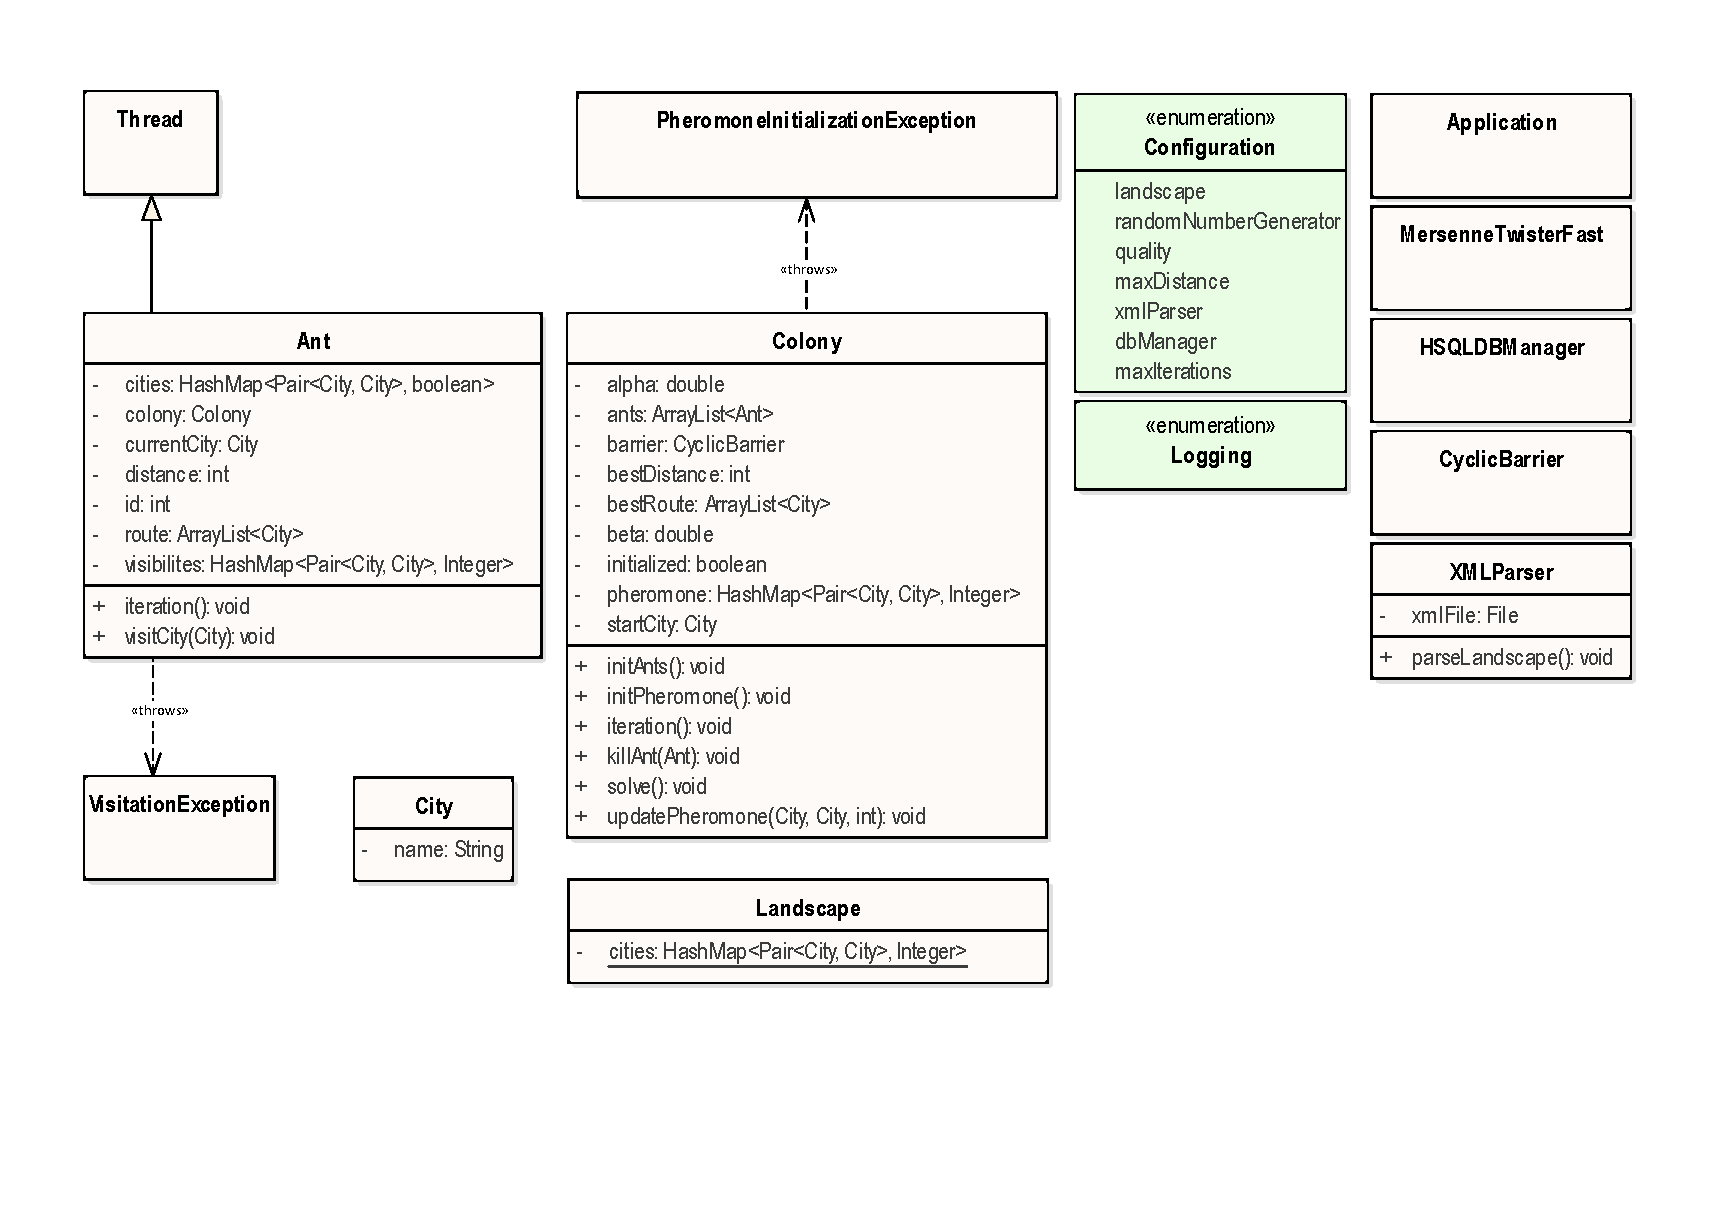
\includegraphics[width=0.9\linewidth]{images/classModel.eps}
		\caption{UML-Modellierung des Architekturentwurfs}
		\label{uml_class}
	\end{figure}

}